\textbf{Paso 1: Estructuración según el patrón MVC}  
Se decidió implementar el patrón Modelo-Vista-Controlador (MVC) para organizar el código y mantener una separación clara de responsabilidades.  
Se crearon tres carpetas principales dentro del proyecto: 

\begin{figure}[H]
    \centering
    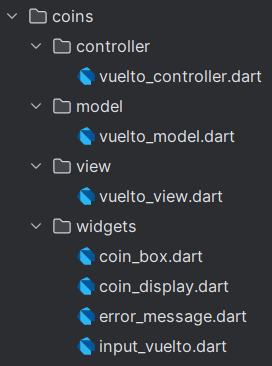
\includegraphics[width=0.4 \textwidth, height=6cm, keepaspectratio]{ej13/cap1.png}
    \caption{Patrón MVC en years}
    \label{fig:ej13il1}
\end{figure}

\textbf{Paso 2: Creación de archivos .dart para cada componente}  
Dentro de cada carpeta se añadieron los archivos correspondientes:  
\begin{itemize}
    \item aniosmodel.dart en model
    \item anioscontroller.dart en controller
    \item aniosview.dart en view
\end{itemize}

\textbf{Paso 3: Desarrollo de los componentes (modelo $\rightarrow$ controlador $\rightarrow$ vista)}  

\textbf{aniosmodel.dart:}  
En este archivo se implementó la lógica para determinar si un año es bisiesto. Se creó la función \texttt{esBisiesto}, que recibe como parámetro un número entero correspondiente al año y devuelve un valor booleano (\texttt{true} o \texttt{false}) según cumpla las condiciones del calendario para años bisiestos.  

El método sigue la regla estándar:  
\begin{itemize}
    \item Un año no divisible entre 4 no es bisiesto.
    \item Un año divisible entre 4 pero no entre 100 sí es bisiesto.
    \item Un año divisible entre 400 también es bisiesto.
\end{itemize}

De esta forma, se encapsula toda la lógica del cálculo en el modelo, separándola de la interfaz y del control.

\textbf{anioscontroller.dart:}  
En este archivo se desarrolló la lógica de control que gestiona la interacción entre el modelo y la vista. La clase \texttt{AnioController} se encarga de recibir el dato ingresado por el usuario, validarlo y devolver un mensaje adecuado según corresponda.  

El método \texttt{procesar} realiza varias funciones:  

\begin{center}
\begin{lstlisting}
class AnioModel {
  //Condicion si es bisiesto
  static bool esBisiesto(int anio){
    if (anio % 4 != 0){
      return false;
    } else if (anio % 100 != 0){
      return true;
    } else if (anio % 400 == 0){
      return true;
    } else {
      return false;
    }
  }
}
\end{lstlisting}
\end{center}

\begin{itemize}
    \item Verifica que el campo no esté vacío.
    \item Comprueba que el valor ingresado sea un número positivo válido.
    \item Controla que el año no exceda un límite máximo definido (\texttt{maxAnio}).
    \item Llama al método \texttt{esBisiesto} del modelo (\texttt{AnioModel}) para determinar si el año es bisiesto o no.
    \item Devuelve un mensaje claro para el usuario indicando si el año es bisiesto o no, o si hubo algún error en la entrada.
\end{itemize}

De esta manera, el controlador centraliza la lógica de validación y procesamiento, manteniendo la separación entre los datos (modelo) y la presentación (vista) y asegurando que la interfaz reciba únicamente la información ya procesada y lista para mostrar.

\textbf{aniosview.dart:}  
En este archivo se construyó la interfaz de usuario de la aplicación, combinando los Widgets necesarios para que el usuario pueda interactuar y verificar si un año es bisiesto.

\begin{center}
\begin{lstlisting}
class AnioController {
  static const int maxAnio = 9999;

  String procesar(String anioStr) {
    if (anioStr.isEmpty) {
      return 'Ingrese un año';
    }

    final anio = int.tryParse(anioStr);
    if (anio == null || anio <= 0) {
      return 'Ingrese un número válido';
    }

    if (anio > maxAnio) {
      return 'Ingrese un año menor o igual a $maxAnio';
    }

    final esBisiesto = AnioModel.esBisiesto(anio);
    if (esBisiesto) {
      return 'El año $anio es bisiesto';
    } else {
      return 'El año $anio no es bisiesto';
    }
  }
}
\end{lstlisting}
\end{center}

Se implementaron distintos componentes reutilizables:  
\begin{itemize}
    \item \textbf{Átomos:} elementos básicos como \texttt{LabelText}, \texttt{ResultText}, \texttt{PrimaryButton} y \texttt{NumberField}. Estos definen estilos y comportamientos individuales.
    \item \textbf{Moléculas:} combinaciones de átomos como \texttt{AnioInput}, que integra un campo de texto para ingresar el año con su formato y validación de entrada.
    \item \textbf{Organismos:} \texttt{AnioCard}, que reúne todos los elementos anteriores (etiqueta, input, botón y resultado) en una sección cohesiva que permite la interacción completa.
\end{itemize}

El componente \texttt{AnioPage} actúa como la página principal, donde se inserta \texttt{AnioCard} dentro de un \texttt{Scaffold} para presentar la interfaz completa.  

\textbf{Paso 4: Integración en la aplicación}  
En el archivo \texttt{Home} se configura la pantalla principal de la aplicación y se gestionan las diferentes secciones mediante un \texttt{NavigationBar} inferior.  

Para la funcionalidad de verificación de años bisiestos:  
\begin{itemize}
    \item Se importa la vista \texttt{AnioPage} para poder mostrarla dentro del contenedor principal de la app.
    \item La página se agrega a la lista de vistas que se despliegan dinámicamente en el \texttt{body} del \texttt{Scaffold}.
    \item El índice \texttt{currentPageIndex} determina qué página se muestra; cuando el usuario selecciona la opción correspondiente a “Bisiesto” en la barra de navegación, se instancia y se despliega \texttt{AnioPage}.
\end{itemize}

De esta manera, \texttt{Home} permite integrar y mostrar la página de años bisiestos de forma organizada.
